% Options for packages loaded elsewhere
% Options for packages loaded elsewhere
\PassOptionsToPackage{unicode}{hyperref}
\PassOptionsToPackage{hyphens}{url}
\PassOptionsToPackage{dvipsnames,svgnames,x11names}{xcolor}
%
\documentclass[
  letterpaper,
  DIV=11,
  numbers=noendperiod]{scrartcl}
\usepackage{xcolor}
\usepackage{amsmath,amssymb}
\setcounter{secnumdepth}{5}
\usepackage{iftex}
\ifPDFTeX
  \usepackage[T1]{fontenc}
  \usepackage[utf8]{inputenc}
  \usepackage{textcomp} % provide euro and other symbols
\else % if luatex or xetex
  \usepackage{unicode-math} % this also loads fontspec
  \defaultfontfeatures{Scale=MatchLowercase}
  \defaultfontfeatures[\rmfamily]{Ligatures=TeX,Scale=1}
\fi
\usepackage{lmodern}
\ifPDFTeX\else
  % xetex/luatex font selection
\fi
% Use upquote if available, for straight quotes in verbatim environments
\IfFileExists{upquote.sty}{\usepackage{upquote}}{}
\IfFileExists{microtype.sty}{% use microtype if available
  \usepackage[]{microtype}
  \UseMicrotypeSet[protrusion]{basicmath} % disable protrusion for tt fonts
}{}
\makeatletter
\@ifundefined{KOMAClassName}{% if non-KOMA class
  \IfFileExists{parskip.sty}{%
    \usepackage{parskip}
  }{% else
    \setlength{\parindent}{0pt}
    \setlength{\parskip}{6pt plus 2pt minus 1pt}}
}{% if KOMA class
  \KOMAoptions{parskip=half}}
\makeatother
% Make \paragraph and \subparagraph free-standing
\makeatletter
\ifx\paragraph\undefined\else
  \let\oldparagraph\paragraph
  \renewcommand{\paragraph}{
    \@ifstar
      \xxxParagraphStar
      \xxxParagraphNoStar
  }
  \newcommand{\xxxParagraphStar}[1]{\oldparagraph*{#1}\mbox{}}
  \newcommand{\xxxParagraphNoStar}[1]{\oldparagraph{#1}\mbox{}}
\fi
\ifx\subparagraph\undefined\else
  \let\oldsubparagraph\subparagraph
  \renewcommand{\subparagraph}{
    \@ifstar
      \xxxSubParagraphStar
      \xxxSubParagraphNoStar
  }
  \newcommand{\xxxSubParagraphStar}[1]{\oldsubparagraph*{#1}\mbox{}}
  \newcommand{\xxxSubParagraphNoStar}[1]{\oldsubparagraph{#1}\mbox{}}
\fi
\makeatother

\usepackage{color}
\usepackage{fancyvrb}
\newcommand{\VerbBar}{|}
\newcommand{\VERB}{\Verb[commandchars=\\\{\}]}
\DefineVerbatimEnvironment{Highlighting}{Verbatim}{commandchars=\\\{\}}
% Add ',fontsize=\small' for more characters per line
\usepackage{framed}
\definecolor{shadecolor}{RGB}{241,243,245}
\newenvironment{Shaded}{\begin{snugshade}}{\end{snugshade}}
\newcommand{\AlertTok}[1]{\textcolor[rgb]{0.68,0.00,0.00}{#1}}
\newcommand{\AnnotationTok}[1]{\textcolor[rgb]{0.37,0.37,0.37}{#1}}
\newcommand{\AttributeTok}[1]{\textcolor[rgb]{0.40,0.45,0.13}{#1}}
\newcommand{\BaseNTok}[1]{\textcolor[rgb]{0.68,0.00,0.00}{#1}}
\newcommand{\BuiltInTok}[1]{\textcolor[rgb]{0.00,0.23,0.31}{#1}}
\newcommand{\CharTok}[1]{\textcolor[rgb]{0.13,0.47,0.30}{#1}}
\newcommand{\CommentTok}[1]{\textcolor[rgb]{0.37,0.37,0.37}{#1}}
\newcommand{\CommentVarTok}[1]{\textcolor[rgb]{0.37,0.37,0.37}{\textit{#1}}}
\newcommand{\ConstantTok}[1]{\textcolor[rgb]{0.56,0.35,0.01}{#1}}
\newcommand{\ControlFlowTok}[1]{\textcolor[rgb]{0.00,0.23,0.31}{\textbf{#1}}}
\newcommand{\DataTypeTok}[1]{\textcolor[rgb]{0.68,0.00,0.00}{#1}}
\newcommand{\DecValTok}[1]{\textcolor[rgb]{0.68,0.00,0.00}{#1}}
\newcommand{\DocumentationTok}[1]{\textcolor[rgb]{0.37,0.37,0.37}{\textit{#1}}}
\newcommand{\ErrorTok}[1]{\textcolor[rgb]{0.68,0.00,0.00}{#1}}
\newcommand{\ExtensionTok}[1]{\textcolor[rgb]{0.00,0.23,0.31}{#1}}
\newcommand{\FloatTok}[1]{\textcolor[rgb]{0.68,0.00,0.00}{#1}}
\newcommand{\FunctionTok}[1]{\textcolor[rgb]{0.28,0.35,0.67}{#1}}
\newcommand{\ImportTok}[1]{\textcolor[rgb]{0.00,0.46,0.62}{#1}}
\newcommand{\InformationTok}[1]{\textcolor[rgb]{0.37,0.37,0.37}{#1}}
\newcommand{\KeywordTok}[1]{\textcolor[rgb]{0.00,0.23,0.31}{\textbf{#1}}}
\newcommand{\NormalTok}[1]{\textcolor[rgb]{0.00,0.23,0.31}{#1}}
\newcommand{\OperatorTok}[1]{\textcolor[rgb]{0.37,0.37,0.37}{#1}}
\newcommand{\OtherTok}[1]{\textcolor[rgb]{0.00,0.23,0.31}{#1}}
\newcommand{\PreprocessorTok}[1]{\textcolor[rgb]{0.68,0.00,0.00}{#1}}
\newcommand{\RegionMarkerTok}[1]{\textcolor[rgb]{0.00,0.23,0.31}{#1}}
\newcommand{\SpecialCharTok}[1]{\textcolor[rgb]{0.37,0.37,0.37}{#1}}
\newcommand{\SpecialStringTok}[1]{\textcolor[rgb]{0.13,0.47,0.30}{#1}}
\newcommand{\StringTok}[1]{\textcolor[rgb]{0.13,0.47,0.30}{#1}}
\newcommand{\VariableTok}[1]{\textcolor[rgb]{0.07,0.07,0.07}{#1}}
\newcommand{\VerbatimStringTok}[1]{\textcolor[rgb]{0.13,0.47,0.30}{#1}}
\newcommand{\WarningTok}[1]{\textcolor[rgb]{0.37,0.37,0.37}{\textit{#1}}}

\usepackage{longtable,booktabs,array}
\newcounter{none} % for unnumbered tables
\usepackage{calc} % for calculating minipage widths
% Correct order of tables after \paragraph or \subparagraph
\usepackage{etoolbox}
\makeatletter
\patchcmd\longtable{\par}{\if@noskipsec\mbox{}\fi\par}{}{}
\makeatother
% Allow footnotes in longtable head/foot
\IfFileExists{footnotehyper.sty}{\usepackage{footnotehyper}}{\usepackage{footnote}}
\makesavenoteenv{longtable}
\usepackage{graphicx}
\makeatletter
\newsavebox\pandoc@box
\newcommand*\pandocbounded[1]{% scales image to fit in text height/width
  \sbox\pandoc@box{#1}%
  \Gscale@div\@tempa{\textheight}{\dimexpr\ht\pandoc@box+\dp\pandoc@box\relax}%
  \Gscale@div\@tempb{\linewidth}{\wd\pandoc@box}%
  \ifdim\@tempb\p@<\@tempa\p@\let\@tempa\@tempb\fi% select the smaller of both
  \ifdim\@tempa\p@<\p@\scalebox{\@tempa}{\usebox\pandoc@box}%
  \else\usebox{\pandoc@box}%
  \fi%
}
% Set default figure placement to htbp
\def\fps@figure{htbp}
\makeatother





\setlength{\emergencystretch}{3em} % prevent overfull lines

\providecommand{\tightlist}{%
  \setlength{\itemsep}{0pt}\setlength{\parskip}{0pt}}



 


\KOMAoption{captions}{tableheading}
\makeatletter
\@ifpackageloaded{caption}{}{\usepackage{caption}}
\AtBeginDocument{%
\ifdefined\contentsname
  \renewcommand*\contentsname{Table of contents}
\else
  \newcommand\contentsname{Table of contents}
\fi
\ifdefined\listfigurename
  \renewcommand*\listfigurename{List of Figures}
\else
  \newcommand\listfigurename{List of Figures}
\fi
\ifdefined\listtablename
  \renewcommand*\listtablename{List of Tables}
\else
  \newcommand\listtablename{List of Tables}
\fi
\ifdefined\figurename
  \renewcommand*\figurename{Figure}
\else
  \newcommand\figurename{Figure}
\fi
\ifdefined\tablename
  \renewcommand*\tablename{Table}
\else
  \newcommand\tablename{Table}
\fi
}
\@ifpackageloaded{float}{}{\usepackage{float}}
\floatstyle{ruled}
\@ifundefined{c@chapter}{\newfloat{codelisting}{h}{lop}}{\newfloat{codelisting}{h}{lop}[chapter]}
\floatname{codelisting}{Listing}
\newcommand*\listoflistings{\listof{codelisting}{List of Listings}}
\makeatother
\makeatletter
\makeatother
\makeatletter
\@ifpackageloaded{caption}{}{\usepackage{caption}}
\@ifpackageloaded{subcaption}{}{\usepackage{subcaption}}
\makeatother
\usepackage{bookmark}
\IfFileExists{xurl.sty}{\usepackage{xurl}}{} % add URL line breaks if available
\urlstyle{same}
% fallback for those not using the hyperref driver hyperxmp:
\makeatletter
\@ifundefined{xmpquote}{\newcommand{\xmpquote}[1]{#1}}{}
\makeatother
\hypersetup{
  pdftitle={Transportation Frequency and Employment Status},
  pdfauthor={Rachel Rapier},
  colorlinks=true,
  linkcolor={blue},
  filecolor={Maroon},
  citecolor={Blue},
  urlcolor={Blue},
  pdfcreator={LaTeX via pandoc}}


\title{Transportation Frequency and Employment Status}
\author{Rachel Rapier}
\date{2025-10-15}
\begin{document}
\maketitle
\begin{abstract}
This manuscript discusses the relationship between public transportation
and rideshare frequency based on employment status and whether the
individual had access to a vehicle.
\end{abstract}

\renewcommand*\contentsname{Table of contents}
{
\setcounter{tocdepth}{3}
\tableofcontents
}

\section{Introduction:}\label{introduction}

The type of transportation an individual chooses to use is influenced by
a variety of factors, including employment status and access to a
vehicle.

A full-time employee working in the office will have to be in the office
20-22 days per month, while part-time employees, contract employees, and
retirees will not need to commute as frequently. Because full time
employees are required to be somewhere more days of the week than other
types of employment, I hypothesize that the sum of their total public
transportation days per month and rideshare days per month will be
higher than those who are not full-time employed. I also hypothesize
that access to a vehicle will decrease the total number of public
transportaion and rideshare rides. I hypothesize that access to a
vehicle will have a stronger effect on the number of public
transportation and rideshare rides for individuals not employed
full-time.

Full time employees may have more disposable income to afford a vehicle.
Others may rely sol

Transportation use and frequency varies based on num between full-time
employed individuals and those who are not employed full-time. In this
study, I examine public transportation and rideshare usage patterns
between these two groups.

In addition, having access to a vehicle can impact transportation
choices, and I hypothesize that access to a vehicle will decrease the \#
of days per month that individuals use public transportation or
rideshare services.

\section{Data and Methods}\label{data-and-methods}

\subsubsection{Standard Package Imports and Data
Loading}\label{standard-package-imports-and-data-loading}

\protect\phantomsection\label{load-packages-data}
\begin{Shaded}
\begin{Highlighting}[]
\ImportTok{import}\NormalTok{ pandas }\ImportTok{as}\NormalTok{ pd}
\ImportTok{import}\NormalTok{ numpy }\ImportTok{as}\NormalTok{ np}
\ImportTok{import}\NormalTok{ matplotlib.pyplot }\ImportTok{as}\NormalTok{ plt}
\ImportTok{import}\NormalTok{ seaborn }\ImportTok{as}\NormalTok{ sns}
\ImportTok{from}\NormalTok{ IPython.display }\ImportTok{import}\NormalTok{ display, Markdown}
\ImportTok{import}\NormalTok{ statsmodels.api }\ImportTok{as}\NormalTok{ sm}
\ImportTok{from}\NormalTok{ statsmodels.formula.api }\ImportTok{import}\NormalTok{ ols}
\ImportTok{from}\NormalTok{ collections }\ImportTok{import}\NormalTok{ defaultdict}

\NormalTok{sns.set\_context(}\StringTok{\textquotesingle{}talk\textquotesingle{}}\NormalTok{)}

\NormalTok{dataA }\OperatorTok{=}\NormalTok{ pd.read\_csv(}\StringTok{\textquotesingle{}data\_orig/PRCAProlificExport\_FileA.csv\textquotesingle{}}\NormalTok{)}
\NormalTok{dataB }\OperatorTok{=}\NormalTok{ pd.read\_csv(}\StringTok{\textquotesingle{}data\_orig/PRCAProlificExport\_FileB.csv\textquotesingle{}}\NormalTok{)}
\NormalTok{dataC }\OperatorTok{=}\NormalTok{ pd.read\_csv(}\StringTok{\textquotesingle{}data\_orig/PRCAQualtricsExport\_FileC.csv\textquotesingle{}}\NormalTok{)}

\NormalTok{questions }\OperatorTok{=}\NormalTok{ pd.read\_csv(}\StringTok{\textquotesingle{}data\_dictionary.csv\textquotesingle{}}\NormalTok{)}


\CommentTok{\# rename the columns to variable\_name and question}
\NormalTok{questions.rename(columns}\OperatorTok{=}\NormalTok{\{questions.columns[}\DecValTok{0}\NormalTok{]: }\StringTok{\textquotesingle{}variable\_name\textquotesingle{}}\NormalTok{, questions.columns[}\DecValTok{1}\NormalTok{]: }\StringTok{\textquotesingle{}question\textquotesingle{}}\NormalTok{\}, inplace}\OperatorTok{=}\VariableTok{True}\NormalTok{)}

\CommentTok{\# merge dataframes}
\NormalTok{data\_all }\OperatorTok{=}\NormalTok{ pd.merge(dataA, dataB, how }\OperatorTok{=} \StringTok{\textquotesingle{}outer\textquotesingle{}}\NormalTok{)}

\CommentTok{\# Then merge the result with dataC (Q0 in dataC contains Participant id that matches Participant id in dataA/dataB)}
\NormalTok{data\_all }\OperatorTok{=}\NormalTok{ pd.merge(data\_all, dataC, left\_on}\OperatorTok{=}\StringTok{\textquotesingle{}Participant id\textquotesingle{}}\NormalTok{, right\_on}\OperatorTok{=}\StringTok{\textquotesingle{}Q0\textquotesingle{}}\NormalTok{, how}\OperatorTok{=}\StringTok{\textquotesingle{}right\textquotesingle{}}\NormalTok{)}
\end{Highlighting}
\end{Shaded}

\textsubscript{Source:
\href{https://RachelRapier.github.io/psych_755_project/index.qmd.html}{Article
Notebook}}

\subsubsection{Data Cleaning}\label{data-cleaning}

I created a new particpant ID as an index that was simplified from the
original dataset. This was done to make the data easier to work with and
to avoid issues with the long string of numbers in the original
participant ID.

I then dropped the columns in the data set that I was not using for my
analysis.

There were 2 participants that completed the survey in less than 30
seconds, so I dropped them from the dataset because their values would
not be accurate.

\textsubscript{Source:
\href{https://RachelRapier.github.io/psych_755_project/index.qmd.html}{Article
Notebook}}

\protect\phantomsection\label{cleaning-data}
\begin{Shaded}
\begin{Highlighting}[]
\CommentTok{\#create an indexing column because participant id a long string of numbers and we want to simplify it. This index will be used as the participant id. Then move it to the first column}

\NormalTok{data\_all[}\StringTok{\textquotesingle{}p\_id\textquotesingle{}}\NormalTok{] }\OperatorTok{=}\NormalTok{ data\_all.index}
\NormalTok{data\_all }\OperatorTok{=}\NormalTok{ data\_all[[}\StringTok{\textquotesingle{}p\_id\textquotesingle{}}\NormalTok{] }\OperatorTok{+}\NormalTok{ [col }\ControlFlowTok{for}\NormalTok{ col }\KeywordTok{in}\NormalTok{ data\_all.columns }\ControlFlowTok{if}\NormalTok{ col }\OperatorTok{!=} \StringTok{\textquotesingle{}p\_id\textquotesingle{}}\NormalTok{]]}

\CommentTok{\#drop columns that are not needed   }
\NormalTok{df }\OperatorTok{=}\NormalTok{ data\_all.drop(columns}\OperatorTok{=}\NormalTok{[}\StringTok{\textquotesingle{}EndDate\textquotesingle{}}\NormalTok{, }\StringTok{\textquotesingle{}StartDate\textquotesingle{}}\NormalTok{, }\StringTok{\textquotesingle{}LocationLatitude\textquotesingle{}}\NormalTok{, }\StringTok{\textquotesingle{}LocationLongitude\textquotesingle{}}\NormalTok{, }\StringTok{\textquotesingle{}Started at\textquotesingle{}}\NormalTok{, }\StringTok{\textquotesingle{}Completed at\textquotesingle{}}\NormalTok{, }\StringTok{\textquotesingle{}ResponseId\textquotesingle{}}\NormalTok{, }\StringTok{\textquotesingle{}Participant id\textquotesingle{}}\NormalTok{, }\StringTok{\textquotesingle{}Submission id\textquotesingle{}}\NormalTok{, }\StringTok{\textquotesingle{}Total approvals\textquotesingle{}}\NormalTok{, }\StringTok{\textquotesingle{}Sex\textquotesingle{}}\NormalTok{, }\StringTok{\textquotesingle{}Country of residence\textquotesingle{}}\NormalTok{, }\StringTok{\textquotesingle{}Student status\textquotesingle{}}\NormalTok{, }\StringTok{\textquotesingle{}Age\textquotesingle{}}\NormalTok{])}

\CommentTok{\#filter for participants that took more than 30 seconds to complete the survey}

\NormalTok{df }\OperatorTok{=}\NormalTok{ df[df[}\StringTok{\textquotesingle{}Duration (in seconds)\textquotesingle{}}\NormalTok{]}\OperatorTok{\textgreater{}} \DecValTok{30}\NormalTok{]}

\NormalTok{df }\OperatorTok{=}\NormalTok{ df.drop(columns}\OperatorTok{=}\NormalTok{[}\StringTok{\textquotesingle{}Duration (in seconds)\textquotesingle{}}\NormalTok{, }\StringTok{\textquotesingle{}Time taken\textquotesingle{}}\NormalTok{])}
\end{Highlighting}
\end{Shaded}

\textsubscript{Source:
\href{https://RachelRapier.github.io/psych_755_project/index.qmd.html}{Article
Notebook}}

I converted the rideshare days per month and the public transportation
days per month variables into numeric values (0-4) and renamed the
columns to be more descriptive. One participant reported `Not Sure' for
acess to a vehicle, so I removed them from the data set. Employment
status was simplified to a binary variable (full-time or other). I
created my dependent variable \texttt{total\_rides} by summing the
rideshare days per month and public transportation days per month
variables.

\textsubscript{Source:
\href{https://RachelRapier.github.io/psych_755_project/index.qmd.html}{Article
Notebook}}

\protect\phantomsection\label{map-numeric-values}
\begin{Shaded}
\begin{Highlighting}[]
\CommentTok{\# Get unique values for each Q column (excluding Q0)}
\NormalTok{q\_unique\_vals }\OperatorTok{=}\NormalTok{ \{\}}
\ControlFlowTok{for}\NormalTok{ col }\KeywordTok{in}\NormalTok{ df.columns:}
    \ControlFlowTok{if}\NormalTok{ col.startswith(}\StringTok{\textquotesingle{}Q\textquotesingle{}}\NormalTok{) }\KeywordTok{and} \KeywordTok{not}\NormalTok{ col.startswith(}\StringTok{\textquotesingle{}Q0\textquotesingle{}}\NormalTok{):}
\NormalTok{        unique\_vals }\OperatorTok{=} \BuiltInTok{tuple}\NormalTok{(}\BuiltInTok{sorted}\NormalTok{(df[col].dropna().unique()))}
\NormalTok{        q\_unique\_vals[col] }\OperatorTok{=}\NormalTok{ unique\_vals}

\CommentTok{\# Group columns by their unique values}
\NormalTok{value\_groups }\OperatorTok{=}\NormalTok{ defaultdict(}\BuiltInTok{list}\NormalTok{)}
\ControlFlowTok{for}\NormalTok{ col, vals }\KeywordTok{in}\NormalTok{ q\_unique\_vals.items():}
\NormalTok{    value\_groups[vals].append(col)}



\NormalTok{group2\_mapping }\OperatorTok{=}\NormalTok{ \{}
  \StringTok{\textquotesingle{}0{-}1 days a month\textquotesingle{}}\NormalTok{: }\DecValTok{1}\NormalTok{, }
  \StringTok{\textquotesingle{}2{-}4 days a month\textquotesingle{}}\NormalTok{: }\DecValTok{2}\NormalTok{, }
  \StringTok{\textquotesingle{}4{-}8 days a month\textquotesingle{}}\NormalTok{: }\DecValTok{3}\NormalTok{, }
  \StringTok{\textquotesingle{}8 or more days a month\textquotesingle{}}\NormalTok{: }\DecValTok{4}\NormalTok{, }
  \StringTok{\textquotesingle{}Never\textquotesingle{}}\NormalTok{: }\DecValTok{0}
\NormalTok{\}}
\NormalTok{group3\_mapping }\OperatorTok{=}\NormalTok{ \{}
  \StringTok{\textquotesingle{}1{-}2 rides in a typical day\textquotesingle{}}\NormalTok{: }\DecValTok{1}\NormalTok{, }
  \StringTok{\textquotesingle{}3{-}4 rides in a typical day\textquotesingle{}}\NormalTok{: }\DecValTok{2}\NormalTok{, }
  \StringTok{\textquotesingle{}5{-}6 rides in a typical day\textquotesingle{}}\NormalTok{: }\DecValTok{3}\NormalTok{, }
  \StringTok{\textquotesingle{}7 or more rides in a typical day\textquotesingle{}}\NormalTok{: }\DecValTok{4}
\NormalTok{\}}

\ControlFlowTok{for}\NormalTok{ col }\KeywordTok{in}\NormalTok{ df.columns:}
    \ControlFlowTok{if}\NormalTok{ col }\KeywordTok{in}\NormalTok{ value\_groups[}\BuiltInTok{tuple}\NormalTok{(}\BuiltInTok{sorted}\NormalTok{(group3\_mapping.keys()))]:}
\NormalTok{        df[col }\OperatorTok{+} \StringTok{\textquotesingle{}\_numeric\textquotesingle{}}\NormalTok{] }\OperatorTok{=}\NormalTok{ df[col].}\BuiltInTok{map}\NormalTok{(group3\_mapping)}

\ControlFlowTok{for}\NormalTok{ col }\KeywordTok{in}\NormalTok{ df.columns:}
    \ControlFlowTok{if}\NormalTok{ col }\KeywordTok{in}\NormalTok{ value\_groups[}\BuiltInTok{tuple}\NormalTok{(}\BuiltInTok{sorted}\NormalTok{(group2\_mapping.keys()))]:}
\NormalTok{        df[col }\OperatorTok{+} \StringTok{\textquotesingle{}\_numeric\textquotesingle{}}\NormalTok{] }\OperatorTok{=}\NormalTok{ df[col].}\BuiltInTok{map}\NormalTok{(group2\_mapping)}

\CommentTok{\#rename the new numeric columns something that makes more sense}
\NormalTok{df }\OperatorTok{=}\NormalTok{ df.rename(columns}\OperatorTok{=}\NormalTok{\{}
  \StringTok{\textquotesingle{}Q26\_numeric\textquotesingle{}}\NormalTok{: }\StringTok{\textquotesingle{}public\_trans\_per\_month\textquotesingle{}}\NormalTok{, }
  \StringTok{\textquotesingle{}Q27\_numeric\textquotesingle{}}\NormalTok{: }\StringTok{\textquotesingle{}public\_trans\_reg\_day\textquotesingle{}}\NormalTok{, }
  \StringTok{\textquotesingle{}Q28\_numeric\textquotesingle{}}\NormalTok{: }\StringTok{\textquotesingle{}rideshare\_per\_month\textquotesingle{}}\NormalTok{, }
  \StringTok{\textquotesingle{}Q29\_numeric\textquotesingle{}}\NormalTok{: }\StringTok{\textquotesingle{}rideshare\_reg\_day\textquotesingle{}}\NormalTok{, }
  \StringTok{\textquotesingle{}Q21\textquotesingle{}}\NormalTok{:}\StringTok{\textquotesingle{}Car Access\textquotesingle{}}\NormalTok{\})}


\CommentTok{\#drop ALL Q columns}
\NormalTok{df }\OperatorTok{=}\NormalTok{ df.drop(columns}\OperatorTok{=}\NormalTok{[col }\ControlFlowTok{for}\NormalTok{ col }\KeywordTok{in}\NormalTok{ df.columns }\ControlFlowTok{if}\NormalTok{ col.startswith(}\StringTok{\textquotesingle{}Q\textquotesingle{}}\NormalTok{)])}

\CommentTok{\#remove 1 participant that has \textquotesingle{}Not Sure\textquotesingle{} as their car access response}
\NormalTok{df }\OperatorTok{=}\NormalTok{ df[df[}\StringTok{\textquotesingle{}Car Access\textquotesingle{}}\NormalTok{] }\OperatorTok{!=} \StringTok{\textquotesingle{}Not Sure\textquotesingle{}}\NormalTok{]}

\CommentTok{\# create a new column called Full{-}Time that combines Part{-}Time and Other into Other for Employment Status}
\NormalTok{df[}\StringTok{\textquotesingle{}Full{-}Time\textquotesingle{}}\NormalTok{] }\OperatorTok{=}\NormalTok{ df[}\StringTok{\textquotesingle{}Employment status\textquotesingle{}}\NormalTok{].}\BuiltInTok{apply}\NormalTok{(}\KeywordTok{lambda}\NormalTok{ x: }\StringTok{\textquotesingle{}Other\textquotesingle{}} \ControlFlowTok{if}\NormalTok{ x }\KeywordTok{in}\NormalTok{ [}\StringTok{\textquotesingle{}Part{-}Time\textquotesingle{}}\NormalTok{, }\StringTok{\textquotesingle{}Other\textquotesingle{}}\NormalTok{] }\ControlFlowTok{else}\NormalTok{ x)}

\CommentTok{\# create my new outcome variable {-} total rides}
\NormalTok{df[}\StringTok{\textquotesingle{}total\_rides\textquotesingle{}}\NormalTok{] }\OperatorTok{=}\NormalTok{ df[}\StringTok{\textquotesingle{}public\_trans\_per\_month\textquotesingle{}}\NormalTok{] }\OperatorTok{+}\NormalTok{ df[}\StringTok{\textquotesingle{}rideshare\_per\_month\textquotesingle{}}\NormalTok{]}


\NormalTok{df }\OperatorTok{=}\NormalTok{ df.drop(columns}\OperatorTok{=}\NormalTok{[}\StringTok{\textquotesingle{}public\_trans\_reg\_day\textquotesingle{}}\NormalTok{, }\StringTok{\textquotesingle{}rideshare\_reg\_day\textquotesingle{}}\NormalTok{])}
\end{Highlighting}
\end{Shaded}

\textsubscript{Source:
\href{https://RachelRapier.github.io/psych_755_project/index.qmd.html}{Article
Notebook}}

\section{Methods and Data}\label{methods-and-data}

\textsubscript{Source:
\href{https://RachelRapier.github.io/psych_755_project/index.qmd.html}{Article
Notebook}}

\protect\phantomsection\label{new_merged_data_info}
\begin{Shaded}
\begin{Highlighting}[]
\BuiltInTok{print}\NormalTok{(}\SpecialStringTok{f"Merged dataframe shape: }\SpecialCharTok{\{}\NormalTok{df}\SpecialCharTok{.}\NormalTok{shape}\SpecialCharTok{\}}\SpecialStringTok{"}\NormalTok{)}
\BuiltInTok{print}\NormalTok{(}\SpecialStringTok{f"Columns in merged dataframe: }\SpecialCharTok{\{}\NormalTok{df}\SpecialCharTok{.}\NormalTok{columns}\SpecialCharTok{.}\NormalTok{tolist()}\SpecialCharTok{\}}\SpecialStringTok{"}\NormalTok{)}
\end{Highlighting}
\end{Shaded}

\begin{verbatim}
Merged dataframe shape: (270, 7)
Columns in merged dataframe: ['p_id', 'Employment status', 'Car Access', 'public_trans_per_month', 'rideshare_per_month', 'Full-Time', 'total_rides']
\end{verbatim}

\textsubscript{Source:
\href{https://RachelRapier.github.io/psych_755_project/index.qmd.html}{Article
Notebook}}

\begin{Shaded}
\begin{Highlighting}[]
\CommentTok{\# Check for any unreasonable values in the dataset}

\CommentTok{\# Create a mapping of variable names to human{-}readable descriptions}
\NormalTok{variable\_descriptions }\OperatorTok{=}\NormalTok{ \{}
    \StringTok{\textquotesingle{}public\_trans\_per\_month\textquotesingle{}}\NormalTok{: }\StringTok{\textquotesingle{}Public Transportation Days per Month\textquotesingle{}}\NormalTok{,}
    \StringTok{\textquotesingle{}rideshare\_per\_month\textquotesingle{}}\NormalTok{: }\StringTok{\textquotesingle{}Rideshare Days per Month\textquotesingle{}}\NormalTok{,}
    \StringTok{\textquotesingle{}total\_rides\textquotesingle{}}\NormalTok{: }\StringTok{\textquotesingle{}Total Ride Days per Month\textquotesingle{}}
\NormalTok{\}}

\CommentTok{\# Get the descriptive statistics and transpose}
\NormalTok{desc\_stats }\OperatorTok{=}\NormalTok{ df.drop(columns }\OperatorTok{=}\NormalTok{ [}\StringTok{\textquotesingle{}p\_id\textquotesingle{}}\NormalTok{]).describe().transpose().}\BuiltInTok{apply}\NormalTok{(}\KeywordTok{lambda}\NormalTok{ x: }\BuiltInTok{round}\NormalTok{(x, }\DecValTok{2}\NormalTok{))}

\CommentTok{\# Add human{-}readable descriptions as a new column}
\NormalTok{desc\_stats[}\StringTok{\textquotesingle{}Variable\textquotesingle{}}\NormalTok{] }\OperatorTok{=}\NormalTok{ desc\_stats.index.}\BuiltInTok{map}\NormalTok{(variable\_descriptions)}

\CommentTok{\# Drop the existing index and set the new column as the index}
\NormalTok{desc\_stats }\OperatorTok{=}\NormalTok{ desc\_stats.reset\_index(drop}\OperatorTok{=}\VariableTok{True}\NormalTok{).set\_index(}\StringTok{\textquotesingle{}Variable\textquotesingle{}}\NormalTok{).drop(columns }\OperatorTok{=}\NormalTok{ [}\StringTok{\textquotesingle{}25\%\textquotesingle{}}\NormalTok{, }\StringTok{\textquotesingle{}50\%\textquotesingle{}}\NormalTok{, }\StringTok{\textquotesingle{}75\%\textquotesingle{}}\NormalTok{])}

\NormalTok{desc\_stats}
\end{Highlighting}
\end{Shaded}

{

\begin{longtable}[]{@{}llllll@{}}

\caption{\label{tbl-describe_dataframe}Descriptive statistics for the
cleaned dataset}

\tabularnewline

\toprule\noalign{}
& count & mean & std & min & max \\
Variable & & & & & \\
\midrule\noalign{}
\endhead
\bottomrule\noalign{}
\endlastfoot
Public Transportation Days per Month & 270.0 & 2.13 & 1.46 & 0.0 &
4.0 \\
Rideshare Days per Month & 270.0 & 1.51 & 1.24 & 0.0 & 4.0 \\
Total Ride Days per Month & 270.0 & 3.63 & 2.35 & 0.0 & 8.0 \\

\end{longtable}

}

\textsubscript{Source:
\href{https://RachelRapier.github.io/psych_755_project/index.qmd.html}{Article
Notebook}}

\begin{Shaded}
\begin{Highlighting}[]
\CommentTok{\# Drop p\_id column}
\NormalTok{df\_plot }\OperatorTok{=}\NormalTok{ df.drop(columns}\OperatorTok{=}\NormalTok{[}\StringTok{\textquotesingle{}p\_id\textquotesingle{}}\NormalTok{])}

\NormalTok{df\_plot.hist(figsize}\OperatorTok{=}\NormalTok{(}\DecValTok{8}\NormalTok{, }\DecValTok{10}\NormalTok{))}
\NormalTok{plt.show()}
\end{Highlighting}
\end{Shaded}

\begin{figure}[H]

\centering{

\pandocbounded{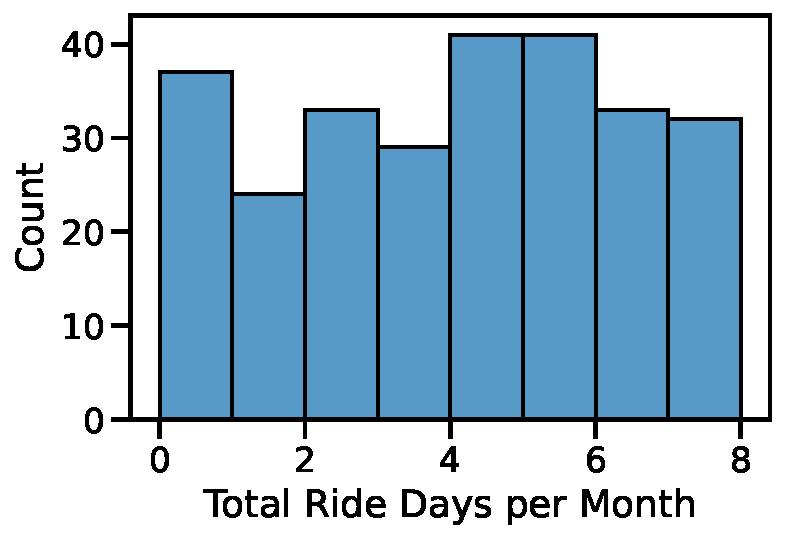
\includegraphics[keepaspectratio]{index_files/figure-pdf/fig-histograms-output-1.pdf}}

}

\caption{\label{fig-histograms}Histograms of numeric variables}

\end{figure}%

\textsubscript{Source:
\href{https://RachelRapier.github.io/psych_755_project/index.qmd.html}{Article
Notebook}}

\subsection{Employment Status}\label{employment-status}

\begin{Shaded}
\begin{Highlighting}[]
\CommentTok{\# Create a mapping of employment status values to human{-}readable descriptions}
\NormalTok{employment\_descriptions }\OperatorTok{=}\NormalTok{ \{}
    \StringTok{\textquotesingle{}Full{-}Time\textquotesingle{}}\NormalTok{: }\StringTok{\textquotesingle{}Full{-}Time Employment\textquotesingle{}}\NormalTok{,}
    \StringTok{\textquotesingle{}Other\textquotesingle{}}\NormalTok{: }\StringTok{\textquotesingle{}Other Employment Status\textquotesingle{}}
\NormalTok{\}}

\CommentTok{\# Get the value counts}
\NormalTok{employ\_counts }\OperatorTok{=}\NormalTok{ df[}\StringTok{\textquotesingle{}Full{-}Time\textquotesingle{}}\NormalTok{].value\_counts()}

\CommentTok{\# Create a DataFrame with the counts}
\NormalTok{employ\_tbl }\OperatorTok{=}\NormalTok{ pd.DataFrame(\{}\StringTok{\textquotesingle{}count\textquotesingle{}}\NormalTok{: employ\_counts\})}

\CommentTok{\# Add human{-}readable descriptions as a new column}
\NormalTok{employ\_tbl[}\StringTok{\textquotesingle{}Employment\textquotesingle{}}\NormalTok{] }\OperatorTok{=}\NormalTok{ employ\_tbl.index.}\BuiltInTok{map}\NormalTok{(employment\_descriptions)}

\CommentTok{\# Drop the existing index and set the new column as the index}
\NormalTok{employ\_tbl }\OperatorTok{=}\NormalTok{ employ\_tbl.reset\_index(drop}\OperatorTok{=}\VariableTok{True}\NormalTok{).set\_index(}\StringTok{\textquotesingle{}Employment\textquotesingle{}}\NormalTok{)}

\NormalTok{employ\_tbl}
\end{Highlighting}
\end{Shaded}

{

\begin{longtable}[]{@{}ll@{}}

\caption{\label{tbl-valuecounts-employment}Value counts for employment
status}

\tabularnewline

\toprule\noalign{}
& count \\
Employment & \\
\midrule\noalign{}
\endhead
\bottomrule\noalign{}
\endlastfoot
Full-Time Employment & 154 \\
Other Employment Status & 97 \\

\end{longtable}

}

\textsubscript{Source:
\href{https://RachelRapier.github.io/psych_755_project/index.qmd.html}{Article
Notebook}}

\textsubscript{Source:
\href{https://RachelRapier.github.io/psych_755_project/index.qmd.html}{Article
Notebook}}

\subsection{Vehicle Access}\label{vehicle-access}

\begin{Shaded}
\begin{Highlighting}[]
\CommentTok{\# Create a mapping of car access values to human{-}readable descriptions}
\NormalTok{VehicleAccess }\OperatorTok{=}\NormalTok{ \{}
    \StringTok{\textquotesingle{}Yes\textquotesingle{}}\NormalTok{: }\StringTok{\textquotesingle{}Has Access to Vehicle\textquotesingle{}}\NormalTok{,}
    \StringTok{\textquotesingle{}No\textquotesingle{}}\NormalTok{: }\StringTok{\textquotesingle{}No Access to Vehicle\textquotesingle{}}
\NormalTok{\}}

\CommentTok{\# Get the value counts}
\NormalTok{car\_counts }\OperatorTok{=}\NormalTok{ df[}\StringTok{\textquotesingle{}Car Access\textquotesingle{}}\NormalTok{].value\_counts()}

\CommentTok{\# Create a DataFrame with the counts}
\NormalTok{car\_tbl }\OperatorTok{=}\NormalTok{ pd.DataFrame(\{}\StringTok{\textquotesingle{}count\textquotesingle{}}\NormalTok{: car\_counts\})}

\CommentTok{\# Add human{-}readable descriptions as a new column}
\NormalTok{car\_tbl[}\StringTok{\textquotesingle{}Vehicle Access\textquotesingle{}}\NormalTok{] }\OperatorTok{=}\NormalTok{ car\_tbl.index.}\BuiltInTok{map}\NormalTok{(VehicleAccess)}

\CommentTok{\# Drop the existing index and set the new column as the index}
\NormalTok{car\_tbl }\OperatorTok{=}\NormalTok{ car\_tbl.reset\_index(drop}\OperatorTok{=}\VariableTok{True}\NormalTok{).set\_index(}\StringTok{\textquotesingle{}Vehicle Access\textquotesingle{}}\NormalTok{)}

\NormalTok{car\_tbl}
\end{Highlighting}
\end{Shaded}

{

\begin{longtable}[]{@{}ll@{}}

\caption{\label{tbl-valuecounts-car}Value counts for car access}

\tabularnewline

\toprule\noalign{}
& count \\
Vehicle Access & \\
\midrule\noalign{}
\endhead
\bottomrule\noalign{}
\endlastfoot
Has Access to Vehicle & 133 \\
No Access to Vehicle & 33 \\

\end{longtable}

}

\textsubscript{Source:
\href{https://RachelRapier.github.io/psych_755_project/index.qmd.html}{Article
Notebook}}

\textsubscript{Source:
\href{https://RachelRapier.github.io/psych_755_project/index.qmd.html}{Article
Notebook}}

\textsubscript{Source:
\href{https://RachelRapier.github.io/psych_755_project/index.qmd.html}{Article
Notebook}}

\begin{Shaded}
\begin{Highlighting}[]
\CommentTok{\# put value count for employmentstats and for car access in the same figure and make the y axis the same for each plot and don\textquotesingle{}t show the y axis for the 2nd plot}
\NormalTok{fig, axes }\OperatorTok{=}\NormalTok{ plt.subplots(}\DecValTok{1}\NormalTok{, }\DecValTok{2}\NormalTok{)}
\NormalTok{df[}\StringTok{\textquotesingle{}Full{-}Time\textquotesingle{}}\NormalTok{].value\_counts().plot(kind}\OperatorTok{=}\StringTok{\textquotesingle{}bar\textquotesingle{}}\NormalTok{, ax}\OperatorTok{=}\NormalTok{axes[}\DecValTok{0}\NormalTok{])}
\NormalTok{df[}\StringTok{\textquotesingle{}Car Access\textquotesingle{}}\NormalTok{].value\_counts().plot(kind}\OperatorTok{=}\StringTok{\textquotesingle{}bar\textquotesingle{}}\NormalTok{, ax}\OperatorTok{=}\NormalTok{axes[}\DecValTok{1}\NormalTok{])}
\NormalTok{axes[}\DecValTok{0}\NormalTok{].set\_ylim([}\DecValTok{0}\NormalTok{, }\DecValTok{160}\NormalTok{])}
\NormalTok{axes[}\DecValTok{1}\NormalTok{].set\_ylim([}\DecValTok{0}\NormalTok{, }\DecValTok{160}\NormalTok{])}
\NormalTok{axes[}\DecValTok{1}\NormalTok{].set\_yticks([])   }\CommentTok{\# Remove y{-}axis ticks for the second plot}
\NormalTok{axes[}\DecValTok{1}\NormalTok{].set\_xlabel(}\StringTok{\textquotesingle{}Car Access\textquotesingle{}}\NormalTok{)}
\NormalTok{plt.title(}\StringTok{\textquotesingle{}Count of Employment Status and Vehicle Access\textquotesingle{}}\NormalTok{)}
\NormalTok{plt.show()}
\end{Highlighting}
\end{Shaded}

\begin{figure}[H]

\centering{

\pandocbounded{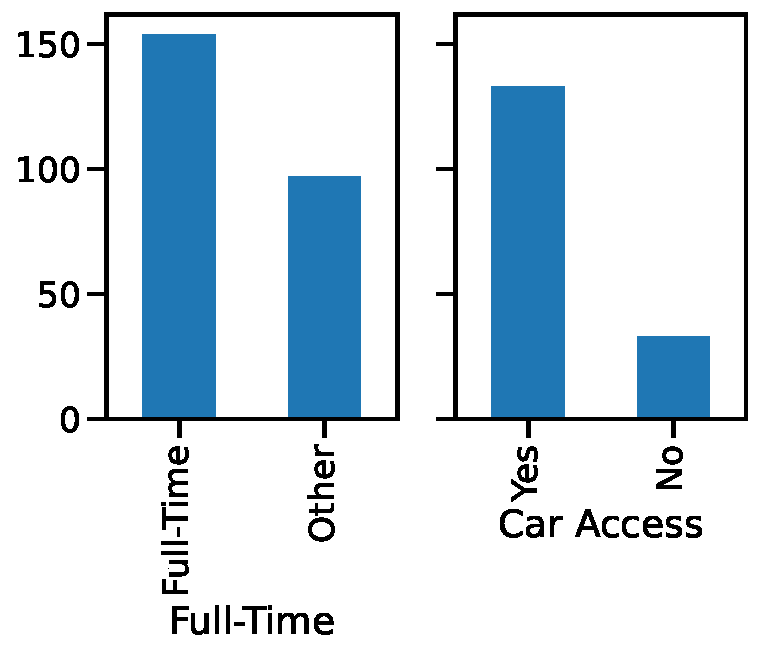
\includegraphics[keepaspectratio]{index_files/figure-pdf/fig-barplot-output-1.pdf}}

}

\caption{\label{fig-barplot}Histograms of Employment Status and Vehicle
Access}

\end{figure}%

\textsubscript{Source:
\href{https://RachelRapier.github.io/psych_755_project/index.qmd.html}{Article
Notebook}}

\section{Results}\label{results}

\textsubscript{Source:
\href{https://RachelRapier.github.io/psych_755_project/index.qmd.html}{Article
Notebook}}

\begin{Shaded}
\begin{Highlighting}[]
\NormalTok{cross\_tab }\OperatorTok{=}\NormalTok{ df.groupby([}\StringTok{\textquotesingle{}Full{-}Time\textquotesingle{}}\NormalTok{, }\StringTok{\textquotesingle{}Car Access\textquotesingle{}}\NormalTok{])[}\StringTok{\textquotesingle{}total\_rides\textquotesingle{}}\NormalTok{].describe().drop(columns }\OperatorTok{=}\NormalTok{ [}\StringTok{\textquotesingle{}25\%\textquotesingle{}}\NormalTok{, }\StringTok{\textquotesingle{}50\%\textquotesingle{}}\NormalTok{, }\StringTok{\textquotesingle{}75\%\textquotesingle{}}\NormalTok{]).}\BuiltInTok{round}\NormalTok{(}\DecValTok{2}\NormalTok{)}
\NormalTok{cross\_tab}
\end{Highlighting}
\end{Shaded}

{

\begin{longtable}[]{@{}lllllll@{}}

\caption{\label{tbl-groupby}Descriptive Statistics for Total Rides by
Employment Status and Vehicle Access}

\tabularnewline

\toprule\noalign{}
& & count & mean & std & min & max \\
Full-Time & Car Access & & & & & \\
\midrule\noalign{}
\endhead
\bottomrule\noalign{}
\endlastfoot
\multirow{2}{*}{Full-Time} & No & 10.0 & 4.80 & 2.04 & 0.0 & 7.0 \\
& Yes & 75.0 & 3.49 & 2.16 & 0.0 & 8.0 \\
\multirow{2}{*}{Other} & No & 16.0 & 4.31 & 1.58 & 2.0 & 8.0 \\
& Yes & 51.0 & 2.14 & 2.14 & 0.0 & 8.0 \\

\end{longtable}

}

\textsubscript{Source:
\href{https://RachelRapier.github.io/psych_755_project/index.qmd.html}{Article
Notebook}}

\begin{Shaded}
\begin{Highlighting}[]
\CommentTok{\# Create the ANOVA model (using Q() for column names with special characters)}
\NormalTok{model }\OperatorTok{=}\NormalTok{ ols(}\StringTok{\textquotesingle{}total\_rides \textasciitilde{} C(Q("Full{-}Time")) * C(Q("Car Access"))\textquotesingle{}}\NormalTok{, data}\OperatorTok{=}\NormalTok{df).fit()}

\CommentTok{\# Get the ANOVA table}
\NormalTok{anova\_table }\OperatorTok{=}\NormalTok{ sm.stats.anova\_lm(model, typ}\OperatorTok{=}\DecValTok{2}\NormalTok{).}\BuiltInTok{round}\NormalTok{(}\DecValTok{2}\NormalTok{)}

\CommentTok{\# Display the ANOVA table}
\NormalTok{anova\_table}
\end{Highlighting}
\end{Shaded}

{

\begin{longtable}[]{@{}lllll@{}}

\caption{\label{tbl-anova}2x2 ANOVA results for total rides by
employment status and vehicle access}

\tabularnewline

\toprule\noalign{}
& sum\_sq & df & F & PR(\textgreater F) \\
\midrule\noalign{}
\endhead
\bottomrule\noalign{}
\endlastfoot
C(Q("Full-Time")) & 53.43 & 1.0 & 12.17 & 0.00 \\
C(Q("Car Access")) & 68.83 & 1.0 & 15.68 & 0.00 \\
C(Q("Full-Time")):C(Q("Car Access")) & 3.86 & 1.0 & 0.88 & 0.35 \\
Residual & 649.82 & 148.0 & NaN & NaN \\

\end{longtable}

}

\textsubscript{Source:
\href{https://RachelRapier.github.io/psych_755_project/index.qmd.html}{Article
Notebook}}

Table~\ref{tbl-describe_dataframe} give general descriptive statistics
of the numeric values of the data.

Table~\ref{tbl-groupby} shows the descriptive statistics of my dependent
variable `total\_rides' by employment status and vehicle access.

\textsubscript{Source:
\href{https://RachelRapier.github.io/psych_755_project/index.qmd.html}{Article
Notebook}}

\begin{Shaded}
\begin{Highlighting}[]
\CommentTok{\#create a boxplot of total\_rides by employment status and vehicle access}
\NormalTok{sns.boxplot(data}\OperatorTok{=}\NormalTok{df, x}\OperatorTok{=}\StringTok{\textquotesingle{}Full{-}Time\textquotesingle{}}\NormalTok{, y}\OperatorTok{=}\StringTok{\textquotesingle{}total\_rides\textquotesingle{}}\NormalTok{, hue}\OperatorTok{=}\StringTok{\textquotesingle{}Car Access\textquotesingle{}}\NormalTok{)}
\NormalTok{plt.title(}\StringTok{\textquotesingle{}Total Rides by Employment Status and Vehicle Access\textquotesingle{}}\NormalTok{)}
\NormalTok{plt.xlabel(}\StringTok{\textquotesingle{}Employment Status\textquotesingle{}}\NormalTok{)}
\NormalTok{plt.ylabel(}\StringTok{\textquotesingle{}Total Rides per Month\textquotesingle{}}\NormalTok{)}
\NormalTok{plt.legend(title}\OperatorTok{=}\StringTok{\textquotesingle{}Vehicle Access\textquotesingle{}}\NormalTok{, bbox\_to\_anchor}\OperatorTok{=}\NormalTok{(}\FloatTok{1.05}\NormalTok{, }\DecValTok{1}\NormalTok{), loc}\OperatorTok{=}\StringTok{\textquotesingle{}upper left\textquotesingle{}}\NormalTok{)}
\NormalTok{plt.tight\_layout()}
\NormalTok{plt.show()}
\end{Highlighting}
\end{Shaded}

\begin{figure}[H]

\centering{

\pandocbounded{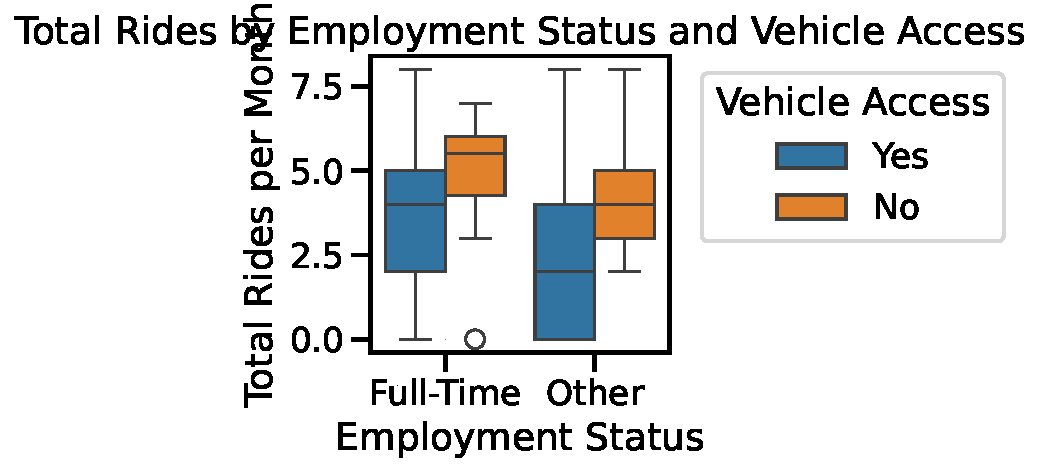
\includegraphics[keepaspectratio]{index_files/figure-pdf/fig-boxplot-output-1.pdf}}

}

\caption{\label{fig-boxplot}Boxplot of total rides by employment status
and vehicle access}

\end{figure}%

\textsubscript{Source:
\href{https://RachelRapier.github.io/psych_755_project/index.qmd.html}{Article
Notebook}}

\section{Conclusion, Future Directions, \&
Limitations}\label{conclusion-future-directions-limitations}

\subsection{Future Directions}\label{future-directions}

Reviewing Figure~\ref{fig-boxplot}, there appears to be an outlier that
is a full-time employee without access to a car with very low ride share
and public transportation usage days. It would be interesting to further
examine this outlier; however, it seems to be this person may walk to
work or work from home.

\subsection{Limitations}\label{limitations}

The distributions of the variables(Figure~\ref{fig-barplot},
Figure~\ref{fig-histograms}) are not normal, which may impact the
results of the ANOVA test.

\textsubscript{Source:
\href{https://RachelRapier.github.io/psych_755_project/index.qmd.html}{Article
Notebook}}




\end{document}
